\documentclass[11pt]{article}
\usepackage[utf8]{inputenc}
\usepackage{amsmath,amssymb,amsthm}
\usepackage{booktabs}
\usepackage{graphicx}
\usepackage{tikz}
\usepackage[margin=0.8in]{geometry}
\usepackage{natbib}
\usepackage{xcolor}
\usepackage[colorlinks=true,linkcolor=blue!60!black,citecolor=blue!60!black,urlcolor=blue!60!black]{hyperref}
\hypersetup{pdftitle={Secular Equation and Exact Loss Convolution for Minibatch Heavy-Ball SGD on Quadratics},pdfauthor={Gabriel Paiva}}
\usepackage[expansion=false]{microtype}

\newtheorem{theorem}{Theorem}
\newtheorem{proposition}[theorem]{Proposition}
\newtheorem{lemma}[theorem]{Lemma}
\newtheorem{corollary}[theorem]{Corollary}
\theoremstyle{remark}
\newtheorem{remark}[theorem]{Remark}

\newcommand{\etacrit}{\eta_{\mathrm{crit}}}
\newcommand{\E}{\mathbb{E}}
\newcommand{\R}{\mathbb{R}}
\newcommand{\Var}{\operatorname{Var}}
\newcommand{\Cov}{\operatorname{Cov}}
\newcommand{\tr}{\operatorname{tr}}
\renewcommand{\labelitemi}{$\bullet$}

\title{Secular Equation and Exact Loss Convolution for Minibatch Heavy-Ball SGD on Quadratics}
\author{Gabriel Paiva\\ \texttt{gabriel@echdesign.co.uk}}
\date{November 2026}

\makeatletter\g@addto@macro\UrlBreaks{\do\-}\makeatother
\begin{document}
\maketitle

\begin{abstract}
For heavy-ball SGD on a quadratic in $\R^P$,
\[
w_{t+1} = \big((1+\beta)I - \eta H_{B_t}\big)w_t - \beta w_{t-1} - \eta \xi_t,
\]
with i.i.d.\ minibatch Hessians $H_{B_t}$ of mean $H \succ 0$, we study the mean-square stability threshold $\eta^\star(\beta)$ and the expected loss at finite $P$. When the minibatch Hessians are formed from random features with independent coordinates in the eigenbasis of $H$ and excess kurtosis $\kappa_{\mathrm{feat}} \ge -2$, $\eta^\star(\beta)$ is the unique root of a rank-one secular equation (Theorem~\ref{thm:secular}), and twice the expected loss, $\E[\langle w_t, H w_t\rangle]$, obeys an exact discrete convolution equation (Proposition~\ref{prop:renewal}). Its kernel sum equals the secular left-hand side (for $\kappa_{\mathrm{feat}}\ge-1$ on the whole stable range), and at $\alpha_{\mathrm{diag}}=1$ with the large-$n$ pool factor of sampling without replacement it has the closed form of the Volterra kernel norm of \citet{lee2022minibatch}. The reduction uses the threshold for Hessians that need not commute, $\eta^\star(\beta) = 1/\lambda_{\max}(\mathcal L_0^{-1/2}\mathcal B_\beta\mathcal L_0^{-1/2})$ (Theorem~\ref{thm:general}), obtained independently of \citet[Theorem~F.1]{cai2026llm}, which gives the same criterion.
\end{abstract}

\section{Introduction}

Consider heavy-ball stochastic gradient descent on a quadratic loss in $\R^P$ with mean Hessian $H = \sum_{k=1}^P \lambda_k u_k u_k^\top \succ 0$ ($\lambda_1 \ge \dots \ge \lambda_P > 0$):
\begin{equation}\label{eq:hbP}
w_{t+1} = \big((1+\beta)I - \eta H_{B_t}\big)w_t - \beta w_{t-1} - \eta \xi_t, \qquad \beta \in [0,1),\ \eta > 0,
\end{equation}
where $(H_{B_t}, \xi_t)$ are i.i.d.\ across steps with $\E[H_{B_t}] = H$, $\E\|H_{B_t}\|_F^2 < \infty$, $\E[\xi_t] = 0$, $\E[\xi_t \xi_t^\top] = \Sigma_\xi \succeq 0$, and curvature-noise operator
\[
\mathcal V(X) \triangleq \E\big[(H_{B_t} - H) X (H_{B_t} - H)\big] \quad (X \in \mathbb S^P).
\]
For SGD without momentum ($\beta = 0$), \citet{mulayoff2024exact} characterized the exact mean-square stability threshold at interpolating minima as the reciprocal of the top eigenvalue of a symmetrizable operator on $\mathbb S^P$. With momentum $\beta \in (0,1)$, the state space doubles to $(w_t, w_{t-1}) \in \R^{2P}$. In high-dimensional limits where the effective rank $\tr(H)/\lambda_1$ is large, \citet{paquette2021momentum}, \citet{lee2022minibatch}, and \citet{cheng2024highdim} showed that the quadratic risk concentrates on a deterministic Volterra integral equation; in particular, the proof of Proposition~2 of \citet{lee2022minibatch} gives a closed-form expression for the norm of the Volterra kernel under orthogonally invariant data. With non-degenerate additive noise, bounded second moments of a linear recursion with i.i.d.\ coefficients are equivalent to $\rho(\E[F_t\otimes F_t])<1$ \citep[Chapter~3]{costa2005mjls}. For momentum LMS with Gaussian inputs at batch size $1$, \citet{roy1990momentum} derive a necessary condition of the form of the secular equation of Section~\ref{sec:secular}, and \citet{velikanov2023view} obtain a loss-convergence condition of that form under their spectrally expressible approximation. With momentum at finite $P$, \citet{andreyev2026momentum} give the threshold exactly in one dimension and, in $P$ dimensions, expand the Schur complement of the second-moment operator on $2P \times 2P$ matrices for small $\eta$ in the noise-dominated regime, where stability depends only on the effective step $\eta/(1-\beta)$ \citep[the rescaling of][]{yuan2016momentum}. They list the precise instability criterion of SGD with momentum as open, also for nonlinear networks; for the linear recursion \eqref{eq:hbP} the exact threshold is not a function of $\eta/(1-\beta)$ alone (Corollary~\ref{cor:etaeff}). \citet{sharma2026outer} give an exact mean-square criterion for outer Nesterov momentum. Concurrently and independently, \citet[Theorem~F.1]{cai2026llm} give the criterion of Theorem~\ref{thm:general}; their eq.~(67) gives Corollary~\ref{cor:etaeff} without strictness.

In this note we derive, at finite $P$, a secular equation for the threshold and an exact convolution equation for the loss, and connect them to the high-dimensional Volterra kernel:
\begin{enumerate}
\item \textbf{Threshold for non-commuting Hessians (Section~\ref{sec:general}).} Eliminating the lag-one covariance closes the stationary equation on $\Sigma_0$ with a double commutator $[H,[H,\Sigma_0]]$ (Theorem~\ref{thm:lyap}); a cone-preserving factorization reduces stability to a symmetric eigenvalue problem on $\mathbb S^P$ (Theorem~\ref{thm:general}), and $\eta^\star(\beta)/(1-\beta)$ increases strictly with $\beta$ (Corollary~\ref{cor:etaeff}).
\item \textbf{Secular equation and finite-$P$ convolution equation for the loss (Section~\ref{sec:secular}).} For random-feature minibatches with independent coordinates in the eigenbasis of $H$ and fourth moment $3+\kappa_{\mathrm{feat}} \ge 1$, the diagonal of $\Sigma_0$ decouples from the off-diagonal and the threshold is the unique root of a scalar secular equation (Theorem~\ref{thm:secular}). Twice the expected loss, $\ell_t = \tr(H\E[w_t w_t^\top])$, satisfies an exact discrete convolution equation at finite $P$ (Proposition~\ref{prop:renewal}); under the condition of Proposition~\ref{prop:renewal}, which for $\kappa_{\mathrm{feat}}\ge-1$ covers the whole stable range, the kernel sum is the left side of the secular equation, and at $\alpha_{\mathrm{diag}}=1$ with the pool factor of sampling without replacement it has the closed form of the Volterra kernel norm of \citet{lee2022minibatch}.
\item \textbf{Cross-mode coupling vs.\ one-dimensional stability (Section~\ref{sec:numerics}).} For Rademacher features ($\kappa_{\mathrm{feat}} = -2$), the directional curvature $u_1^\top H_{B_t} u_1$ is deterministic, so the one-dimensional threshold along $u_1$ equals the deterministic bound $2(1+\beta)/\lambda_1$ at every batch size $B$, whereas off-diagonal mode coupling $\lambda_1\lambda_k/B$ lowers the true threshold to $O((1-\beta)B/\tr H)$ at high effective rank.
\end{enumerate}

\section{General Non-Commuting Minibatch Hessians}\label{sec:general}

Write $\Sigma_0 = \E[w_t w_t^\top]$, $D_\Theta = \E[(w_{t+1}-w_t)(w_{t+1}-w_t)^\top]$, and $[X,Y] = XY - YX$.

\begin{theorem}[Stationary covariance equation]\label{thm:lyap}
In any covariance-stationary regime of \eqref{eq:hbP} with $\E[w_t] = 0$ and no commutation assumption on $H_{B_t}$:
\begin{enumerate}
\item[(1)] $D_\Theta = \frac{\eta}{1+\beta}(H\Sigma_0 + \Sigma_0 H)$.
\item[(2)] $\Sigma_0$ satisfies the exact matrix equation
\begin{equation}\label{eq:lyap}
(H\Sigma_0 + \Sigma_0 H) - \frac{\eta}{1+\beta}H\Sigma_0 H + \frac{\eta\beta}{(1-\beta)(1-\beta^2)}[H,[H,\Sigma_0]] - \frac{\eta}{1-\beta}\mathcal V(\Sigma_0) = \frac{\eta}{1-\beta}\Sigma_\xi.
\end{equation}
\end{enumerate}
\end{theorem}
\begin{proof}
Let $A = (1+\beta)I - \eta H$ and $\Sigma_1 = \E[w_{t+1}w_t^\top]$. Conditioning on $\mathcal F_{t-1}$, the $\sigma$-field of $(w_0,w_{-1})$ and $(H_{B_s},\xi_s)_{s\le t-1}$, gives $\E[w_{t+1}\mid \mathcal F_{t-1}] = A w_t - \beta w_{t-1}$; multiplying on the right by $w_t^\top$ yields $\Sigma_1 = A\Sigma_0 - \beta\Sigma_1^\top$ and, by transposition, $\Sigma_1^\top = \Sigma_0 A - \beta\Sigma_1$. Solving for $\Sigma_1$ gives
\[
\Sigma_1 = \frac{A\Sigma_0 - \beta\Sigma_0 A}{1-\beta^2}, \qquad \Sigma_1 + \Sigma_1^\top = \frac{A\Sigma_0 + \Sigma_0 A}{1+\beta} = 2\Sigma_0 - \frac{\eta}{1+\beta}(H\Sigma_0 + \Sigma_0 H),
\]
which gives (1) since $D_\Theta = 2\Sigma_0 - \Sigma_1 - \Sigma_1^\top$. For (2), expanding $\Sigma_0 = \E[w_{t+1}w_{t+1}^\top]$ with $w_{t+1} = Aw_t - \beta w_{t-1} - \eta(H_{B_t}-H)w_t - \eta\xi_t$ the cross terms vanish because $(H_{B_t}-H,\xi_t)$ is independent of $(w_t,w_{t-1})$ with zero mean and $\E[w_t]=0$, which gives
\[
\Sigma_0 = A\Sigma_0 A + \beta^2 \Sigma_0 - \beta(A\Sigma_1 + \Sigma_1^\top A) + \eta^2 \mathcal V(\Sigma_0) + \eta^2 \Sigma_\xi.
\]
Since $A^2\Sigma_0 + \Sigma_0 A^2 - 2\beta A\Sigma_0 A = [A,[A,\Sigma_0]] + 2(1-\beta)A\Sigma_0 A$ and $[A,[A,\Sigma_0]] = \eta^2[H,[H,\Sigma_0]]$, substituting $\Sigma_1$ yields
\[
(1-\beta^2)\Sigma_0 - \frac{1-\beta}{1+\beta}A\Sigma_0 A = -\frac{\beta\eta^2}{1-\beta^2}[H,[H,\Sigma_0]] + \eta^2\mathcal V(\Sigma_0) + \eta^2\Sigma_\xi.
\]
Expanding $A\Sigma_0 A = (1+\beta)^2\Sigma_0 - \eta(1+\beta)(H\Sigma_0+\Sigma_0 H) + \eta^2 H\Sigma_0 H$ and dividing by $\eta(1-\beta)$ gives \eqref{eq:lyap}.
\end{proof}

Let $s_t = (w_t, w_{t-1}) \in \R^{2P}$ and $Q_t = \E[s_t s_t^\top] \in \mathbb S^{2P}_+$. The transition matrix of \eqref{eq:hbP} is $F_t = \begin{pmatrix}(1+\beta)I - \eta H_{B_t} & -\beta I \\ I & 0\end{pmatrix}$, and the second-moment operator is $\mathcal T(Q) = \E[F_t Q F_t^\top]$.

\begin{lemma}[Reduction to $\mathbb S^{2P}$ and instability criterion]\label{lem:russodye}
The operator $\mathcal T$ preserves $\mathbb S^{2P}$ and $\mathbb S^{2P}_+$, satisfies $\|\mathcal T^k\| = \|\mathcal T^k(I)\|$ in the operator norm induced by the spectral norm on $\R^{2P\times 2P}$, and has $\rho(\mathcal T) = \rho(\mathcal T|_{\mathbb S^{2P}})$. When $\Sigma_\xi \succ 0$ and either $\xi_t$ is independent of $H_{B_t}$ or $\E[s_0] = 0$, $\sup_{t\ge 0}\E\|w_t\|^2 < \infty$ if and only if $\rho(\mathcal T) < 1$; if $\rho(\mathcal T) \ge 1$, then $\E\|w_t\|^2 + \E\|w_{t-1}\|^2 \ge c t$ for all $t \ge 1$ with $c > 0$.
\end{lemma}
The equivalence of bounded second moments and $\rho(\mathcal T)<1$ is standard \citep[Chapter~3]{costa2005mjls}; Lemma~\ref{lem:russodye} adds the linear lower bound.
\begin{proof}
Since $\mathcal T(Q)^\top = \mathcal T(Q^\top)$ and $\mathcal T^k$ is positive in Kraus form, the Russo--Dye theorem gives $\|\mathcal T^k\| = \|\mathcal T^k(I)\|$ with $\mathcal T^k(I) \in \mathbb S^{2P}_+$, so $\rho(\mathcal T) = \lim_{k\to\infty}\|\mathcal T^k(I)\|^{1/k} = \rho(\mathcal T|_{\mathbb S^{2P}})$. Under the noise assumption, $Q_{t+1} = \mathcal T(Q_t) + G$ with $G = \operatorname{blkdiag}(\eta^2\Sigma_\xi, 0)$. If $\rho(\mathcal T) < 1$, $Q_t = \mathcal T^t(Q_0) + \sum_{s<t}\mathcal T^s(G)$ is bounded. Conversely, by the finite-dimensional Krein--Rutman theorem \citep[Thm.~1.3.2]{berman1994}, the adjoint $\mathcal T^*(Y) = \E[F_t^\top Y F_t]$ on $\mathbb S^{2P}$ has a nonzero eigenmatrix $W \in \mathbb S^{2P}_+$ with eigenvalue $\rho(\mathcal T)$. Its upper-left block $W_{11}$ is nonzero (otherwise $W = \operatorname{blkdiag}(0, W_{22})$ and $F_t^\top W F_t = \operatorname{blkdiag}(W_{22},0)$ would force $W=0$). Thus $g = \tr(W G) = \eta^2\tr(W_{11}\Sigma_\xi) > 0$, and $\tr(W Q_{t+1}) = \rho(\mathcal T)\tr(W Q_t) + g \ge \tr(W Q_t) + g$ whenever $\rho(\mathcal T) \ge 1$, so $\tr(W Q_t) \ge t g$ by induction from $\tr(W Q_0) \ge 0$, giving $\tr Q_t \ge (g/\tr W)t$.
\end{proof}

We now reduce $\rho(\mathcal T) < 1$ from $\mathbb S^{2P}$ to $\mathbb S^P$. Define the deterministic operator
\[
\mathcal L_{\eta,\beta}(X) \triangleq (HX + XH) - \frac{\eta}{1+\beta}HXH + \frac{\eta\beta}{(1-\beta)(1-\beta^2)}[H,[H,X]]
\]
on $\mathbb S^P$. In the eigenbasis of $H$, $\mathcal L_{\eta,\beta}$ is diagonal, multiplying entry $(j,k)$ by
\[
\ell_{jk}(\eta,\beta) = (\lambda_j + \lambda_k) - \frac{\eta\lambda_j\lambda_k}{1+\beta} + \frac{\eta\beta(\lambda_j-\lambda_k)^2}{(1-\beta)(1-\beta^2)},
\]
which is strictly positive for all $\eta \in (0, \eta_{\mathrm{det}})$, where $\eta_{\mathrm{det}} \triangleq \frac{2(1+\beta)}{\lambda_1}$.

\begin{theorem}[Exact mean-square threshold for arbitrary per-sample Hessians]\label{thm:general}
Let $H \succ 0$ and $\mathcal V(X) = \E[(H_{B_t}-H)X(H_{B_t}-H)] \ne 0$. For $\eta \in (0, \eta_{\mathrm{det}})$, set $\mathcal K_{\eta,\beta}(X) \triangleq \frac{\eta}{1-\beta}\mathcal L_{\eta,\beta}^{-1}(\mathcal V(X))$ on $\mathbb S^P$, and define
\[
\mathcal L_0(X) \triangleq HX + XH, \qquad \mathcal B_\beta(X) \triangleq \frac{1}{1+\beta}HXH - \frac{\beta}{(1-\beta)(1-\beta^2)}[H,[H,X]] + \frac{1}{1-\beta}\mathcal V(X).
\]
\begin{enumerate}
\item[(1)] For every $\eta \in (0, \eta_{\mathrm{det}})$, $\mathcal L_{\eta,\beta}^{-1}$ and $\mathcal K_{\eta,\beta}$ preserve the cone $\mathbb S^P_+$, $\rho(\mathcal K_{\eta,\beta})$ is the top eigenvalue of the variational quotient
\begin{equation}\label{eq:rayleigh}
\rho(\mathcal K_{\eta,\beta}) = \frac{1}{1-\beta}\max_{X \in \mathbb S^P \setminus \{0\}} \frac{\tr\big(X\mathcal V(X)\big)}{\sum_{j,k=1}^P \big(\ell_{jk}(\eta,\beta)/\eta\big) (u_j^\top X u_k)^2},
\end{equation}
which increases strictly and continuously with $\eta \in (0, \eta_{\mathrm{det}})$, and $\rho(\mathcal T) < 1 \iff \rho(\mathcal K_{\eta,\beta}) < 1$.
\item[(2)] The mean-square stability threshold $\eta^\star(\beta) \triangleq \sup\{\eta > 0 : \rho(\mathcal T) < 1\}$ is given exactly by
\begin{equation}\label{eq:etastar-general}
\eta^\star(\beta) = \frac{1}{\lambda_{\max}\!\big(\mathcal L_0^{-1/2}\mathcal B_\beta \mathcal L_0^{-1/2}\big)} \le \eta_{\mathrm{det}},
\end{equation}
where $\mathcal L_0^{-1/2}\mathcal B_\beta \mathcal L_0^{-1/2}$ is self-adjoint on $(\mathbb S^P, \langle X,Y\rangle_F = \tr(XY))$. If $(H_{B_t}-H)P_1 \not\equiv 0$ for the orthogonal projector $P_1$ onto $\ker(H-\lambda_1 I)$, then $\lim_{\eta \uparrow \eta_{\mathrm{det}}}\rho(\mathcal K_{\eta,\beta}) = +\infty$ and $\eta^\star(\beta) < \eta_{\mathrm{det}}$ is the unique root of $\rho(\mathcal K_{\eta,\beta}) = 1$.
\end{enumerate}
\end{theorem}
As $(1-\beta)\tr(X\mathcal B_\beta(X))/\tr(X\mathcal L_0(X))$ is the quotient $q_{H,\beta}(X)$ of \citet{cai2026llm}, \eqref{eq:etastar-general} is their Theorem~F.1.
\begin{proof}
(1) Decompose $\mathcal T = \mathcal T_0 + \Delta$ on $\mathbb S^{2P}$ into the mean part $\mathcal T_0(Q) = \bar F Q \bar F^\top$ ($\bar F = \E[F_t]$) and the noise part $\Delta(Q) = \operatorname{blkdiag}(\eta^2\mathcal V(Q_{11}), 0)$. For $\eta \in (0,\eta_{\mathrm{det}})$, $\rho(\mathcal T_0) = \rho(\bar F)^2 < 1$, and $(I-\mathcal T_0)^{-1} = \sum_{t\ge 0}\mathcal T_0^t$ preserves $\mathbb S^{2P}_+$. For any $Y \in \mathbb S^P_+$, the matrix $Q = (I-\mathcal T_0)^{-1}\operatorname{blkdiag}(\eta^2 Y, 0) \in \mathbb S^{2P}_+$ is the stationary covariance of \eqref{eq:hbP} with $\mathcal V = 0$ and $\Sigma_\xi = Y$, so Theorem~\ref{thm:lyap}(2) gives $Q_{11} = \frac{\eta}{1-\beta}\mathcal L_{\eta,\beta}^{-1}(Y) \in \mathbb S^P_+$. Thus $\mathcal L_{\eta,\beta}^{-1}$ preserves $\mathbb S^P_+$. Writing $\Pi(Q) = Q_{11}$ and $\mathcal J(X) = (I-\mathcal T_0)^{-1}\operatorname{blkdiag}(\eta^2\mathcal V(X),0)$, we obtain $(I-\mathcal T_0)^{-1}\Delta = \mathcal J \circ \Pi$ and $\Pi \circ \mathcal J = \mathcal K_{\eta,\beta}$. Since $\mathcal J\circ\Pi$ and $\Pi\circ\mathcal J$ share the same nonzero eigenvalues, $\rho((I-\mathcal T_0)^{-1}\Delta) = \rho(\mathcal K_{\eta,\beta})$, and by regular splitting on the cone $\mathbb S^{2P}_+$ \citep{berman1994}, $\rho(\mathcal T) < 1 \iff \rho((I-\mathcal T_0)^{-1}\Delta) < 1 \iff \rho(\mathcal K_{\eta,\beta}) < 1$. Because $\mathcal N_{\eta,\beta} = \eta\mathcal L_{\eta,\beta}^{-1} \succ 0$ and $\mathcal V$ are self-adjoint on $(\mathbb S^P, \langle\cdot,\cdot\rangle_F)$, $\mathcal K_{\eta,\beta}$ is similar to the symmetric operator $\frac{1}{1-\beta}\mathcal N_{\eta,\beta}^{1/2}\mathcal V\mathcal N_{\eta,\beta}^{1/2}$ and preserves $\mathbb S^P_+$; by the Krein--Rutman theorem \citep{krein1948linear}, $\rho(\mathcal K_{\eta,\beta}) = \lambda_{\max}(\mathcal K_{\eta,\beta})$ is given by \eqref{eq:rayleigh}. Since $\tr(I_P\mathcal V(I_P)) = \E\|H_{B_t}-H\|_F^2 > 0$ and each weight $\ell_{jk}(\eta,\beta)/\eta = (\lambda_j+\lambda_k)/\eta - \frac{\lambda_j\lambda_k}{1+\beta} + \frac{\beta(\lambda_j-\lambda_k)^2}{(1-\beta)(1-\beta^2)}$ decreases strictly with $\eta$, $\rho(\mathcal K_{\eta,\beta})$ is strictly increasing in $\eta$.

(2) Since $\mathcal L_{\eta,\beta} = \mathcal L_0 - \eta\mathcal B_\beta + \frac{\eta}{1-\beta}\mathcal V$, we have $\rho(\mathcal K_{\eta,\beta}) < 1 \iff \lambda_{\max}(\mathcal N_{\eta,\beta}^{1/2}\frac{\mathcal V}{1-\beta}\mathcal N_{\eta,\beta}^{1/2}) < 1 \iff \mathcal L_0 - \eta\mathcal B_\beta \succ 0 \iff \eta\lambda_{\max}(\mathcal L_0^{-1/2}\mathcal B_\beta\mathcal L_0^{-1/2}) < 1$. For $\eta \ge \eta_{\mathrm{det}}$, $\mathcal T \succeq \mathcal T_0$ on $\mathbb S^{2P}_+$ gives $\rho(\mathcal T) \ge \rho(\mathcal T_0) \ge 1$; testing $X = u_1 u_1^\top$ gives $\tr(X\mathcal B_\beta(X))/\tr(X\mathcal L_0(X)) \ge 1/\eta_{\mathrm{det}}$, so \eqref{eq:etastar-general} holds in all cases. As $\eta \uparrow \eta_{\mathrm{det}}$, $\ell_{11}(\eta,\beta)/\eta \asymp \eta_{\mathrm{det}} - \eta \downarrow 0$, so testing $X = s P_1 + \mathcal V(P_1)$ with $s=(\ell_{11}/\eta)^{-1/3}$ in \eqref{eq:rayleigh} gives $\rho(\mathcal K_{\eta,\beta}) \to +\infty$ whenever $(H_{B_t}-H)P_1 \not\equiv 0$ (then $\tr\mathcal V(P_1)>0$, the numerator grows at least like $2s\|\mathcal V(P_1)\|_F^2$, and the denominator stays bounded).
\end{proof}

At $\beta = 0$, \eqref{eq:etastar-general} has the form of Theorem~5 of \citet{mulayoff2024exact}, which they prove at interpolating minima for sampling without replacement (with a pseudo-inverse); here $H\succ0$. For minibatches of size $B$ drawn from $N$ fixed per-sample Hessians $H_1,\dots,H_N$ with mean $H$, $\mathcal V(X) = p\,\frac{1}{N}\sum_{i=1}^N (H_i-H)X(H_i-H)$ with $p = 1/B$ for sampling with replacement and $p = \frac{N-B}{B(N-1)}$ for sampling without replacement.

\begin{corollary}[Strict monotonicity of the effective step at the threshold]\label{cor:etaeff}
If $H \succ 0$ and $\mathcal V$ does not depend on $\beta$, the effective threshold $\eta^\star_{\mathrm{eff}}(\beta) \triangleq \eta^\star(\beta)/(1-\beta)$ increases strictly with $\beta \in [0,1)$ and satisfies
\begin{equation}\label{eq:etaeff-bound}
\frac{1}{\eta^\star(0)} - \frac{1-\beta}{\eta^\star(\beta)} \ge \frac{\beta}{1+\beta}\lambda_{\min}(H).
\end{equation}
\end{corollary}
\begin{proof}
By \eqref{eq:etastar-general}, $1/\eta^\star_{\mathrm{eff}}(\beta) = \lambda_{\max}(\mathcal L_0^{-1/2}\mathcal A_\beta\mathcal L_0^{-1/2})$ with $\mathcal A_\beta = (1-\beta)\mathcal B_\beta$. The noise operator $\mathcal V$ cancels in $\mathcal B_0 - \mathcal A_\beta = \frac{2\beta}{1+\beta}H(\cdot)H + \frac{\beta}{1-\beta^2}[H,[H,\cdot]]$, which is diagonal in the eigenbasis of $H$ with entries $m_{jk}(\beta) = \frac{2\beta}{1+\beta}\lambda_j\lambda_k + \frac{\beta}{1-\beta^2}(\lambda_j-\lambda_k)^2$. Since $m_{jk}(\beta)$ increases strictly on $[0,1)$ and $\lambda_j\lambda_k > 0$, $\mathcal L_0^{-1/2}(\mathcal A_{\beta_1} - \mathcal A_{\beta_2})\mathcal L_0^{-1/2} \succ 0$ for $\beta_1 < \beta_2$, so Weyl's inequality gives $\eta^\star_{\mathrm{eff}}(\beta_2) > \eta^\star_{\mathrm{eff}}(\beta_1)$. Using $m_{jk}(\beta) \ge \frac{\beta}{1+\beta}(\lambda_j^2+\lambda_k^2) \ge \frac{\beta}{1+\beta}\lambda_{\min}(H)(\lambda_j+\lambda_k)$ gives $\mathcal L_0^{-1/2}(\mathcal B_0 - \mathcal A_\beta)\mathcal L_0^{-1/2} \succeq \frac{\beta}{1+\beta}\lambda_{\min}(H)I$ and hence \eqref{eq:etaeff-bound}.
\end{proof}

\section{Random-Feature Minibatches and the Expected Loss}\label{sec:secular}

Suppose now that $H_{B_t} = \frac{1}{B}\sum_{b=1}^B z_{t,b}z_{t,b}^\top$ with $z_{t,b} = H^{1/2}\omega_{t,b}$ drawn afresh and independently for every $(t,b)$, where the coordinates $\omega_k$ of $\omega$ in the eigenbasis of $H$ are independent with $\E[\omega_k] = 0$, $\E[\omega_k^2] = 1$, and $\E[\omega_k^4] = 3 + \kappa_{\mathrm{feat}}$ for $\kappa_{\mathrm{feat}} \ge -2$ ($\kappa_{\mathrm{feat}} = 0$ for Gaussian features, $\kappa_{\mathrm{feat}} = -2$ for Rademacher features $\omega_k \in \{\pm 1\}$). Write $\kappa_\beta = \frac{1+\beta}{1-\beta}$ and $\alpha_{\mathrm{diag}} = 1 + p\kappa_\beta(1+\kappa_{\mathrm{feat}})$, with $p = 1/B$.

\begin{theorem}[Rank-one secular equation]\label{thm:secular}
In the random-feature model above with $\sigma_{\xi,k}^2 = u_k^\top \Sigma_\xi u_k > 0$, the action of $\mathcal V$ on $X \in \mathbb S^P$ in the eigenbasis of $H$ is
\begin{equation}\label{eq:V-rf}
\mathcal V(X)_{kk} = p\lambda_k\tr(HX) + p(1+\kappa_{\mathrm{feat}})\lambda_k^2 X_{kk}, \qquad \mathcal V(X)_{jk} = p\lambda_j\lambda_k X_{jk} \quad (j \ne k).
\end{equation}
Consequently, the off-diagonal entries of $\Sigma_0$ decouple from the diagonal, the normalized diagonal step variances $c_k = \eta^{-2}u_k^\top D_\Theta u_k$ solve, for $\eta<\eta^\star(\beta)$, the M-matrix system
\[
\Big[I - \frac{\eta}{2(1+\beta)}\big(\alpha_{\mathrm{diag}}\Lambda + p\kappa_\beta \lambda\mathbf 1^\top\big)\Big]c = \frac{(\sigma_{\xi,k}^2)_{k=1}^P}{1-\beta^2}, \qquad \Lambda = \operatorname{diag}(\lambda_1,\dots,\lambda_P),
\]
and the mean-square threshold $\eta^\star(\beta)$ is the unique root with $\eta\lambda_1\max(\alpha_{\mathrm{diag}},0) < 2(1+\beta)$ of the secular equation
\begin{equation}\label{eq:secular}
\frac{\eta p}{2(1-\beta)}\sum_{k=1}^P \frac{\lambda_k}{1 - \frac{\eta\lambda_k}{2(1+\beta)}\alpha_{\mathrm{diag}}} = 1.
\end{equation}
Moreover, $\eta^\star(\beta) \le \frac{2(1+\beta)}{\lambda_1\max(\alpha_{\mathrm{diag}},1)}$, strictly when $\alpha_{\mathrm{diag}}>1$, and $\mu^\star \triangleq 2(1+\beta)/\eta^\star(\beta)$ satisfies the two-sided bounds
\begin{equation}\label{eq:sandwich}
\max(\alpha_{\mathrm{diag}},0)\lambda_1 + p\kappa_\beta\tr H \ge \mu^\star \ge \max\Big(\alpha_{\mathrm{diag}}\lambda_1 + p\kappa_\beta\lambda_1,\ \min(\alpha_{\mathrm{diag}},0)\lambda_1 + p\kappa_\beta\tr H\Big).
\end{equation}
\end{theorem}
\begin{proof}
Since $\Cov(\omega_j\omega_l, \omega_m\omega_k)$ is $1$ when $j=m\ne l=k$ or $j=k\ne l=m$, $2+\kappa_{\mathrm{feat}}$ when $j=l=m=k$, and $0$ otherwise, expanding $\mathcal V(X) = p\,\E[(zz^\top - H)X(zz^\top - H)]$ gives \eqref{eq:V-rf}. By \eqref{eq:V-rf}, $\mathcal L_0$ and $\mathcal B_\beta$ leave the diagonal subspace of $\mathbb S^P$ invariant and multiply each off-diagonal entry $(j,k)$ ($j \ne k$) by $\lambda_j+\lambda_k$ and by $b_{jk}=\frac{1+p\kappa_\beta}{1+\beta}\lambda_j\lambda_k-\frac{\beta(\lambda_j-\lambda_k)^2}{(1-\beta)(1-\beta^2)}\le\frac{1+p\kappa_\beta}{1+\beta}\lambda_j\lambda_k$. On the diagonal subspace $X = \operatorname{diag}(\gamma_0)$ with $\gamma_{0,k} = \frac{\eta(1+\beta)}{2\lambda_k}c_k$, the $(k,k)$ entry of \eqref{eq:lyap} reads $\big[I - \frac{\eta}{2(1+\beta)}\mathcal M\big]c = \frac{(\sigma_{\xi,k}^2)_{k=1}^P}{1-\beta^2}$, where $\mathcal M = \alpha_{\mathrm{diag}}\Lambda + p\kappa_\beta\lambda\mathbf 1^\top$ is similar to $\widetilde{\mathcal M} = \alpha_{\mathrm{diag}}\Lambda + p\kappa_\beta\sqrt\lambda\sqrt\lambda^\top$. The off-diagonal entries are never less stable than the diagonal block: for $j\ne k$, the test vector $v=(e_j+e_k)/\sqrt2$ gives $\lambda_{\max}(\widetilde{\mathcal M})\ge v^\top\widetilde{\mathcal M}v=(\alpha_{\mathrm{diag}}+p\kappa_\beta)\frac{\lambda_j+\lambda_k}{2}+p\kappa_\beta\sqrt{\lambda_j\lambda_k}\ge(1+p\kappa_\beta)\frac{2\lambda_j\lambda_k}{\lambda_j+\lambda_k}\ge\frac{2(1+\beta)\,b_{jk}}{\lambda_j+\lambda_k}$, because $\alpha_{\mathrm{diag}}+p\kappa_\beta=1+p\kappa_\beta(2+\kappa_{\mathrm{feat}})\ge1$ (this is where $\kappa_{\mathrm{feat}}\ge-2$ is used) and the arithmetic and geometric means of $\lambda_j,\lambda_k$ are at least their harmonic mean. Hence the top eigenvalue of $\mathcal L_0^{-1/2}\mathcal B_\beta\mathcal L_0^{-1/2}$ is that of the diagonal block, $\lambda_{\max}(\widetilde{\mathcal M})/(2(1+\beta))$, and Theorem~\ref{thm:general} gives $\eta^\star(\beta)=2(1+\beta)/\lambda_{\max}(\widetilde{\mathcal M})$. By the rank-one determinant identity
\[
\det(\mu I - \widetilde{\mathcal M}) = \prod_{k=1}^P (\mu - \alpha_{\mathrm{diag}}\lambda_k)\left(1 - p\kappa_\beta\sum_{k=1}^P \frac{\lambda_k}{\mu - \alpha_{\mathrm{diag}}\lambda_k}\right),
\]
$\mu^\star = \lambda_{\max}(\widetilde{\mathcal M})$ is the unique root of \eqref{eq:secular} with $\mu = 2(1+\beta)/\eta > \max(\alpha_{\mathrm{diag}},0)\lambda_1$; since $e_1^\top\widetilde{\mathcal M}e_1 = (\alpha_{\mathrm{diag}}+p\kappa_\beta)\lambda_1 \ge \lambda_1$, also $\mu^\star \ge \lambda_1$, which gives the upper bound on $\eta^\star(\beta)$. Replacing $\alpha_{\mathrm{diag}}\lambda_k$ in each denominator of \eqref{eq:secular} by $\max(\alpha_{\mathrm{diag}},0)\lambda_1$ or $\min(\alpha_{\mathrm{diag}},0)\lambda_1$, or keeping only the $k=1$ term, gives \eqref{eq:sandwich}.
\end{proof}

\begin{proposition}[Finite-$P$ convolution equation for the expected loss]\label{prop:renewal}
In the setting of Theorem~\ref{thm:secular} with $\Sigma_\xi$ diagonal in the eigenbasis of $H$, $w_0 = w_{-1} = 0$, and $\eta < \eta_{\mathrm{det}}$, let $g_k(0) = 1$, $g_k(1) = 1+\beta-\eta\lambda_k$, and $g_k(\tau+1) = (1+\beta-\eta\lambda_k)g_k(\tau) - \beta g_k(\tau-1)$ be the deterministic impulse response of mode $k$, let $\psi_k(\tau) = \eta^2 g_k(\tau)^2$, and let $h_k$ solve the scalar convolution equation $h_k(\tau) = \psi_k(\tau) + p(1+\kappa_{\mathrm{feat}})\lambda_k^2\sum_{u<\tau}\psi_k(\tau-1-u)h_k(u)$. Then twice the expected loss, $\ell_t \triangleq \tr(H\E[w_t w_t^\top])$, satisfies the exact discrete convolution equation
\begin{equation}\label{eq:renewal}
\ell_t = f_t + \sum_{s=0}^{t-1} K_{t-1-s}\,\ell_s, \qquad K_\tau = p\sum_{k=1}^P \lambda_k^2 h_k(\tau), \qquad f_t = \sum_{k=1}^P \lambda_k \sigma_{\xi,k}^2 \sum_{\tau < t} h_k(\tau).
\end{equation}
Whenever $\eta\lambda_1\max(\alpha_{\mathrm{diag}}, 2-\alpha_{\mathrm{diag}}) < 2(1+\beta)$, the kernel $K_\tau$ is summable and its sum is the left-hand side of the secular equation \eqref{eq:secular}:
\begin{equation}\label{eq:kernelsum}
\sum_{\tau=0}^\infty K_\tau = \frac{\eta p}{2(1-\beta)}\sum_{k=1}^P \frac{\lambda_k}{1 - \frac{\eta\lambda_k}{2(1+\beta)}\alpha_{\mathrm{diag}}}.
\end{equation}
For $\kappa_{\mathrm{feat}}\ge-1$ this condition holds on $(0,\eta^\star(\beta)]$, so $\eta^\star(\beta)$ is the root of $\sum_\tau K_\tau=1$. For $\kappa_{\mathrm{feat}}\in[-2,-1)$ it can fail below $\eta^\star(\beta)$ (e.g.\ $P=2$, $\lambda=(1,0.05)$, $\beta=0$, $B=1$, Rademacher: $\eta^\star=2/1.05$, condition only for $\eta<1$); the threshold is still that of Theorem~\ref{thm:secular}.
\end{proposition}
\begin{proof}
Iterating $Q_{t+1} = \mathcal T_0(Q_t) + \Delta(Q_t) + G$ from $Q_0 = 0$ gives $Q_t = \sum_{s<t}\mathcal T_0^{t-1-s}(\Delta(Q_s)+G)$. Since $(\bar F^\tau)_{11} = \operatorname{diag}(g_k(\tau))$ in the eigenbasis of $H$, \eqref{eq:V-rf} implies that $x_{t,k} = (\E[w_t w_t^\top])_{kk}$ obeys
\[
x_{t,k} = \sum_{s=0}^{t-1} \psi_k(t-1-s)\big(\sigma_{\xi,k}^2 + p\lambda_k \ell_s + p(1+\kappa_{\mathrm{feat}})\lambda_k^2 x_{s,k}\big).
\]
By definition of $h_k$, $x_{t,k} = \sum_{s<t}h_k(t-1-s)(\sigma_{\xi,k}^2 + p\lambda_k\ell_s)$; multiplying by $\lambda_k$ and summing over $k$ yields \eqref{eq:renewal}. By the Yule--Walker identity for the second-order autoregression $g_k$, $\Psi_k \triangleq \sum_{\tau=0}^\infty \psi_k(\tau) = \frac{\eta}{2(1-\beta)\lambda_k(1 - \eta\lambda_k/(2(1+\beta)))}$. When $|p(1+\kappa_{\mathrm{feat}})\lambda_k^2|\Psi_k < 1$ (which is $\eta\lambda_k\max(\alpha_{\mathrm{diag}}, 2-\alpha_{\mathrm{diag}}) < 2(1+\beta)$), the Neumann series for $h_k$ converges absolutely with $\sum_{\tau=0}^\infty h_k(\tau) = \Psi_k / \big(1 - p(1+\kappa_{\mathrm{feat}})\lambda_k^2\Psi_k\big)$, and summing $p\lambda_k^2\sum_\tau h_k(\tau)$ over $k$ gives \eqref{eq:kernelsum}. For $\kappa_{\mathrm{feat}}\ge-1$, $\alpha_{\mathrm{diag}}\ge1$ and $\mu^\star>\alpha_{\mathrm{diag}}\lambda_1$ give $\eta^\star\lambda_1\alpha_{\mathrm{diag}}<2(1+\beta)$. In the example, $\alpha_{\mathrm{diag}}=0$, $\mu^\star=1.05$, and $|p(1+\kappa_{\mathrm{feat}})\lambda_1^2|\Psi_1<1$ only for $\eta<1$.
\end{proof}

\paragraph{Connection to the high-dimensional Volterra equation of \citet{lee2022minibatch} and momentum LMS.}
For large $n$ and $d$ under orthogonal invariance of the data, \citet{lee2022minibatch} describe the loss of minibatch SGD with momentum by a Volterra equation; their Proposition~2 gives conditions, among them $\gamma<(1+\Delta)/(\zeta\sigma_{\max}^2)$, for $\|\mathcal K\|<1$. Under the dictionary $\eta = \gamma B$, $\beta = \Delta$, $\lambda_j = \sigma_j^2/n$ and $\zeta=B/n$ (their update sums the $B$ gradients whereas \eqref{eq:hbP} averages them), the kernel sum \eqref{eq:kernelsum} at $\alpha_{\mathrm{diag}} = 1$, with $p$ replaced by $(1-\zeta)/B$, the large-$n$ form of the without-replacement factor $\frac{n-B}{B(n-1)}$, becomes
\[
\frac{1}{n}\sum_{j=1}^P \frac{(1-\zeta)\gamma\sigma_j^2(1+\Delta)}{(1-\Delta)(2(1+\Delta) - \gamma\zeta\sigma_j^2)},
\]
which is the closed-form kernel norm $\|\mathcal K\|$ in the proof of their Proposition~2; their step condition reads $\eta\lambda_1<1+\beta$, half the deterministic threshold. The two formulas coincide, not the two settings: the pool factor is outside Theorem~\ref{thm:secular} (fresh features), both data classes contain Gaussian data, and their statement is asymptotic while Proposition~\ref{prop:renewal} is exact at finite $P$. With $B=\zeta n$ at fixed $\beta$ and $\zeta$, $\alpha_{\mathrm{diag}} - 1 = p\kappa_\beta(1+\kappa_{\mathrm{feat}}) = O(1/n)$; at finite $P$ and $B$, $\alpha_{\mathrm{diag}}$ is what Theorem~\ref{thm:secular} adds to that formula. At the opposite extreme $B = 1$ with Gaussian inputs ($\kappa_{\mathrm{feat}} = 0$, $\alpha_{\mathrm{diag}} = 1+\kappa_\beta$), \eqref{eq:secular} with $\eta=2\mu$ and $\beta=\alpha$ in their notation coincides with the Schur--Cohn condition $Q(1) > 0$ derived as necessary for momentum LMS by \citet[eqs.~(31)--(33)]{roy1990momentum}; Theorem~\ref{thm:secular} proves that it is also sufficient for mean-square stability when $2\mu\lambda_k<1-\alpha^2$ for every $k$, the region below the first pole of \eqref{eq:secular}.

\section{Asymptotic Regimes and Rademacher Separation}\label{sec:numerics}

The sandwich \eqref{eq:sandwich} captures two distinct regimes of the secular equation \eqref{eq:secular}:
\begin{itemize}
\item \textbf{Large batch / low effective rank ($p\kappa_\beta\tr H/\lambda_1 \ll 1$):} $\eta^\star(\beta) = \frac{2(1+\beta)}{\lambda_1}\big(1 - p\kappa_\beta(2+\kappa_{\mathrm{feat}}) + O(p^2)\big)$ for fixed $H$ with $\lambda_1 > \lambda_2$ as $p\to0$, the $O(p^2)$ term depending on the spectral gap through $\sum_{k\ge2}\lambda_k/(\lambda_1-\lambda_k)$, recovering the deterministic ceiling $2(1+\beta)/\lambda_1$.
\item \textbf{Small batch / high effective rank ($p\kappa_\beta\tr H/\lambda_1 \gg 1$, $\lambda_1/\tr H \to 0$):} $\eta^\star(\beta) = \frac{2(1-\beta)}{p\tr H}\big(1 + o(1)\big)$, governed by $\tr H$ rather than $\lambda_1$; \citet{wang2026momentum} obtain a critical-rate scaling of this form, $\min\{1,B(1-\beta)\}$, for one-pass power-law kernel regression.
\end{itemize}

Theorem~\ref{thm:secular} has a consequence for Rademacher features ($\kappa_{\mathrm{feat}} = -2$). Along the top eigenvector $u_1$, the directional curvature is $u_1^\top H_{B_t} u_1 = \lambda_1 \frac{1}{B}\sum_{b=1}^B \omega_{t,b,1}^2 \equiv \lambda_1$ because $\omega_1^2 \equiv 1$. Hence the directional curvature variance $\nu_{11,B}^2 = \Var(u_1^\top H_{B_t} u_1)$ vanishes identically, and the one-dimensional stability threshold along $\operatorname{span}(u_1)$ \citep{wu2018sgd,andreyev2026momentum},
\begin{equation}\label{eq:1d}
\eta_{\mathrm{crit}}^{\mathrm{1D}}(\beta, B) = \frac{2(1+\beta)/\lambda_1}{1 + \kappa_\beta \nu_{11,B}^2/\lambda_1^2},
\end{equation}
equals the deterministic threshold $2(1+\beta)/\lambda_1$ for every batch size $B$. Yet off-diagonal curvature fluctuations $(u_1^\top H_{B_t} u_k)^2$ have mean $\lambda_1\lambda_k/B > 0$ for $k \ge 2$ and couple the modes: by \eqref{eq:sandwich}, the true threshold satisfies $\eta^\star(\beta) \le \frac{2(1+\beta)}{\lambda_1 + \kappa_\beta\tr(H_\perp)/B}$ for $B \le \kappa_\beta$, where $\tr(H_\perp) = \tr H - \lambda_1$.

\begin{figure}[!ht]
\centering
\resizebox{0.74\textwidth}{!}{% Generated by paper/figures/make-fig-phase1.py from evidence/mean-square-boundary/raw-phase1.json; do not edit.
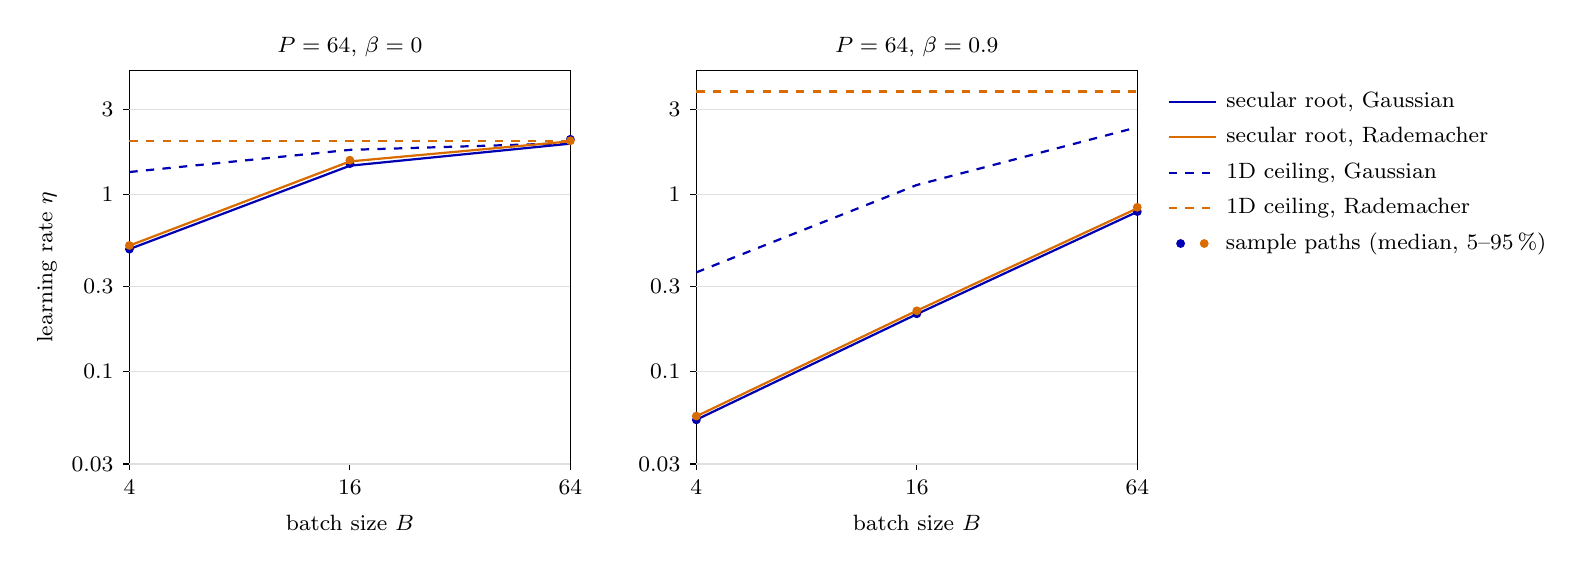
\begin{tikzpicture}[font=\footnotesize]
\tikzset{gauss/.style={blue!70!black}, radem/.style={orange!85!black}}
\draw (0.0,0) rectangle (5.6,5.0);
\draw (0.0000,0) -- (0.0000,-0.08) node[below] {4};
\draw (2.8000,0) -- (2.8000,-0.08) node[below] {16};
\draw (5.6000,0) -- (5.6000,-0.08) node[below] {64};
\draw[gray!25] (0.0,0.0000) -- (5.6,0.0000);
\draw (0.0,0.0000) -- (-0.08,0.0000) node[left] {0.03};
\draw[gray!25] (0.0,1.1767) -- (5.6,1.1767);
\draw (0.0,1.1767) -- (-0.08,1.1767) node[left] {0.1};
\draw[gray!25] (0.0,2.2504) -- (5.6,2.2504);
\draw (0.0,2.2504) -- (-0.08,2.2504) node[left] {0.3};
\draw[gray!25] (0.0,3.4271) -- (5.6,3.4271);
\draw (0.0,3.4271) -- (-0.08,3.4271) node[left] {1};
\draw[gray!25] (0.0,4.5008) -- (5.6,4.5008);
\draw (0.0,4.5008) -- (-0.08,4.5008) node[left] {3};
\node at (2.8,-0.75) {batch size $B$};
\node[anchor=south] at (2.8,5.05) {$P=64$, $\beta=0$};
\node[rotate=90] at (-1.05,2.5) {learning rate $\eta$};
\draw[gauss, dashed, thick] (0.0000,3.7082) -- (2.8000,3.9894) -- (5.6000,4.0744);
\draw[gauss, thick] (0.0000,2.7292) -- (2.8000,3.7880) -- (5.6000,4.0681);
\draw[gauss] (0.0000,2.7249) -- (0.0000,2.7412);
\fill[gauss] (0.0000,2.7287) circle (1.6pt);
\draw[gauss] (2.8000,3.7900) -- (2.8000,3.8213);
\fill[gauss] (2.8000,3.8143) circle (1.6pt);
\draw[gauss] (5.6000,4.0972) -- (5.6000,4.1238);
\fill[gauss] (5.6000,4.1238) circle (1.6pt);
\draw[radem, dashed, thick] (0.0000,4.1045) -- (2.8000,4.1045) -- (5.6000,4.1045);
\draw[radem, thick] (0.0000,2.7735) -- (2.8000,3.8426) -- (5.6000,4.0977);
\draw[radem] (0.0000,2.7730) -- (0.0000,2.7807);
\fill[radem] (0.0000,2.7756) circle (1.6pt);
\draw[radem] (2.8000,3.8425) -- (2.8000,3.8645);
\fill[radem] (2.8000,3.8581) circle (1.6pt);
\draw[radem] (5.6000,4.0979) -- (5.6000,4.1116);
\fill[radem] (5.6000,4.1047) circle (1.6pt);
\draw (7.199999999999999,0) rectangle (12.799999999999999,5.0);
\draw (7.2000,0) -- (7.2000,-0.08) node[below] {4};
\draw (10.0000,0) -- (10.0000,-0.08) node[below] {16};
\draw (12.8000,0) -- (12.8000,-0.08) node[below] {64};
\draw[gray!25] (7.199999999999999,0.0000) -- (12.799999999999999,0.0000);
\draw (7.199999999999999,0.0000) -- (7.119999999999999,0.0000) node[left] {0.03};
\draw[gray!25] (7.199999999999999,1.1767) -- (12.799999999999999,1.1767);
\draw (7.199999999999999,1.1767) -- (7.119999999999999,1.1767) node[left] {0.1};
\draw[gray!25] (7.199999999999999,2.2504) -- (12.799999999999999,2.2504);
\draw (7.199999999999999,2.2504) -- (7.119999999999999,2.2504) node[left] {0.3};
\draw[gray!25] (7.199999999999999,3.4271) -- (12.799999999999999,3.4271);
\draw (7.199999999999999,3.4271) -- (7.119999999999999,3.4271) node[left] {1};
\draw[gray!25] (7.199999999999999,4.5008) -- (12.799999999999999,4.5008);
\draw (7.199999999999999,4.5008) -- (7.119999999999999,4.5008) node[left] {3};
\node at (10.0,-0.75) {batch size $B$};
\node[anchor=south] at (10.0,5.05) {$P=64$, $\beta=0.9$};
\draw[gauss, dashed, thick] (7.2000,2.4337) -- (10.0000,3.5430) -- (12.8000,4.2763);
\draw[gauss, thick] (7.2000,0.5622) -- (10.0000,1.9033) -- (12.8000,3.2026);
\draw[gauss] (7.2000,0.5542) -- (7.2000,0.5696);
\fill[gauss] (7.2000,0.5603) circle (1.6pt);
\draw[gauss] (10.0000,1.8984) -- (10.0000,1.9325);
\fill[gauss] (10.0000,1.9076) circle (1.6pt);
\draw[gauss] (12.8000,3.1915) -- (12.8000,3.2194);
\fill[gauss] (12.8000,3.2054) circle (1.6pt);
\draw[radem, dashed, thick] (7.2000,4.7318) -- (10.0000,4.7318) -- (12.8000,4.7318);
\draw[radem, thick] (7.2000,0.6058) -- (10.0000,1.9469) -- (12.8000,3.2467);
\draw[radem] (7.2000,0.5953) -- (7.2000,0.6166);
\fill[radem] (7.2000,0.6086) circle (1.6pt);
\draw[radem] (10.0000,1.9375) -- (10.0000,1.9615);
\fill[radem] (10.0000,1.9455) circle (1.6pt);
\draw[radem] (12.8000,3.2335) -- (12.8000,3.2685);
\fill[radem] (12.8000,3.2599) circle (1.6pt);
\draw[gauss, thick] (13.2,4.6) -- (13.799999999999999,4.6) node[right, black] {secular root, Gaussian};
\draw[radem, thick] (13.2,4.1499999999999995) -- (13.799999999999999,4.1499999999999995) node[right, black] {secular root, Rademacher};
\draw[gauss, dashed, thick] (13.2,3.6999999999999997) -- (13.799999999999999,3.6999999999999997) node[right, black] {1D ceiling, Gaussian};
\draw[radem, dashed, thick] (13.2,3.2499999999999996) -- (13.799999999999999,3.2499999999999996) node[right, black] {1D ceiling, Rademacher};
\fill[gauss] (13.35,2.8) circle (1.6pt); \fill[radem] (13.649999999999999,2.8) circle (1.6pt);
\node[right] at (13.799999999999999,2.8) {sample paths (median, 5--95\,\%)};
\end{tikzpicture}
}
\caption{Mean-square stability threshold $\eta^\star$ against batch size $B$ for $H = \operatorname{diag}(k^{-1/2})_{k=1}^P$ at $P=64$, $\beta=0$ (left) and $\beta=0.9$ (right). Solid curves: secular root of Theorem~\ref{thm:secular}; dashed curves: one-dimensional threshold \eqref{eq:1d} along $u_1$; dots: median empirical stability threshold over 8 sample-path bisection seeds (5--95\% range); the Gaussian dot at $\beta=0$, $B=64$ is at the bisection cap (Section~\ref{sec:numerics}). Blue: Gaussian features ($\kappa_{\mathrm{feat}}=0$); orange: Rademacher features ($\kappa_{\mathrm{feat}}=-2$), whose one-dimensional threshold along $u_1$ is flat at $2(1+\beta)/\lambda_1$.}
\label{fig:phase1}
\end{figure}

\begin{table}[!ht]
\centering
\caption{Comparison of the one-dimensional threshold \eqref{eq:1d}, the sandwich bounds \eqref{eq:sandwich}, the exact secular root \eqref{eq:secular}, and the median empirical sample-path threshold on $H = \operatorname{diag}(k^{-1/2})_{k=1}^P$ at $\beta = 0.9$. Across all 36 parameter cells tested ($P \in \{64, 256, 1024\}$, $\beta \in \{0, 0.9\}$, $B \in \{4, 16, 64\}$), the crossing $\rho(\mathcal T) = 1$ of the exact second-moment operator agrees with the secular root to at most $6.11 \times 10^{-10}$ relative error, with the operator built from \eqref{eq:V-rf}. The last column divides the one-dimensional threshold by the unrounded secular root.}
\label{tab:rademacher}
\smallskip
{\small
\begin{tabular}{rrlrrrrrr}
\toprule
$P$ & $B$ & Features & $\eta_{\mathrm{crit}}^{\mathrm{1D}}$ & Lower \eqref{eq:sandwich} & Secular $\eta^\star$ & Upper \eqref{eq:sandwich} & Empirical & $\eta_{\mathrm{crit}}^{\mathrm{1D}} / \eta^\star$ \\
\midrule
64  & 4  & Gaussian   & 0.3619 & 0.0506 & 0.0533 & 0.0548 & 0.0532 & $6.8\times$ \\
64  & 4  & Rademacher & 3.8000 & 0.0548 & 0.0558 & 0.0579 & 0.0559 & $68.2\times$ \\
64  & 16 & Gaussian   & 1.1259 & 0.1946 & 0.2103 & 0.2191 & 0.2113 & $5.4\times$ \\
64  & 16 & Rademacher & 3.8000 & 0.2191 & 0.2199 & 0.2215 & 0.2196 & $17.3\times$ \\
64  & 64 & Gaussian   & 2.3843 & 0.6747 & 0.7948 & 0.8766 & 0.7971 & $3.0\times$ \\
64  & 64 & Rademacher & 3.8000 & 0.7543 & 0.8315 & 0.8766 & 0.8428 & $4.6\times$ \\
256 & 4  & Gaussian   & 0.3619 & 0.0252 & 0.0260 & 0.0262 & 0.0261 & $13.9\times$ \\
256 & 4  & Rademacher & 3.8000 & 0.0262 & 0.0263 & 0.0269 & 0.0264 & $144.5\times$ \\
256 & 16 & Gaussian   & 1.1259 & 0.0987 & 0.1034 & 0.1047 & 0.1039 & $10.9\times$ \\
256 & 16 & Rademacher & 3.8000 & 0.1047 & 0.1048 & 0.1052 & 0.1051 & $36.3\times$ \\
\bottomrule
\end{tabular}}
\end{table}

Figure~\ref{fig:phase1} and Table~\ref{tab:rademacher} illustrate Theorem~\ref{thm:secular} on $H = \operatorname{diag}(k^{-1/2})_{k=1}^P$. At $P=256$, $\beta=0.9$, $B=4$ with Rademacher features, the one-dimensional threshold along $u_1$ is $\eta_{\mathrm{crit}}^{\mathrm{1D}} = 3.8$, whereas the secular root is $\eta^\star = 0.0263$ and the empirical sample-path ceiling is $0.0264$; the one-dimensional threshold exceeds the secular root by a factor $144.5$. Sample paths need not track the mean square: at $P=64$, $\beta=0$, $B=64$ with Gaussian features the median bisection run stops at its cap $1.02\cdot2/\lambda_1$, above the secular root $1.9268$ (median $2.003$ with a raised cap), consistent with stable typical paths and a mean square diverging through rare paths; an importance-resampling estimate of the growth of $\E\|w_t\|^2$ crosses $1$ at a median step (8 seeds) $0.32\%$ above the secular root. Code and numerical verification scripts for all results in this note are available at \url{https://github.com/apis-os/hb-sgd-mean-square}.

\renewcommand{\bibfont}{\footnotesize}\setlength{\bibsep}{0pt}
\bibliographystyle{plainnat}
\bibliography{refs}

\end{document}
